\documentclass[12pt,a4paper,openright,twoside]{report}

\usepackage[italian]{babel}
\usepackage[T1]{fontenc}
\usepackage[utf8]{inputenc}

\usepackage{fancyhdr}
\usepackage{indentfirst}
\usepackage[pdftex]{graphicx}
\usepackage{newlfont}

\usepackage{amssymb}
\usepackage{amsmath}
\usepackage{latexsym}
\usepackage{amsthm}

\oddsidemargin=30pt \evensidemargin=20pt%impostano i margini
\usepackage[htt]{hyphenat} %per andare a capo nei typescript
\hyphenation{sil-la-ba-zio-ne pa-ren-te-si}%serve per la sillabazione: tra parentesi 

\pagestyle{fancy}\addtolength{\headwidth}{20pt}
\renewcommand{\chaptermark}[1]{\markboth{\thechapter.\ #1}{}}
\renewcommand{\sectionmark}[1]{\markright{\thesection \ #1}{}}
\rhead[\fancyplain{}{\bfseries\leftmark}]{\fancyplain{}{\bfseries\thepage}}
\cfoot{}

\linespread{1.3}                       

\begin{document}
	
	\cleartorightpage
\thispagestyle{empty}

\vspace*{-1.5cm}
\begin{center}
  \large
  \textbf{ALMA MATER STUDIORUM - UNIVERSITA DI BOLOGNA}\\
  
  \hrulefill\\
  
  \textbf{SCUOLA DI INGEGNERIA  E ARCHITETTURA}\\
  \vspace*{.75cm}
  
  
  Dipartimento di Informatica - Scienza e Ingegneria - DISI\\
  Corso di Laurea Triennale in Ingegneria Informatica\\
  
  \vspace*{1.2cm}
  
  
  \textbf{TESI DI LAUREA}\\
  \vspace*{.4cm}
  in\\
  \vspace*{.4cm}
  LABORATORIO DI AMMINISTRAZIONE DI SISTEMI\\

  \vspace*{2cm} \LARGE
  \textbf{Analisi e sviluppo di un gestore di dati personali secondo il modello MyData}\\
 \end{center}
 
 \vspace*{3cm}
 
 \begin{flushleft}
  \textbf{CANDIDATO}\\ Giada Martina Stivala \\
\end{flushleft}

\vspace*{-2cm}

 \begin{flushright}
  \textbf{RELATORE}\\ Chiar.mo Prof. Marco Prandini \\
  \vspace*{1.5cm}
  \textbf{CORRELATORE}\\ Dott. Andrea Melis
 \end{flushright}

   



\vspace*{2cm}

\begin{center}
	\textbf{
  Anno Accademico 2016/17\\
  Sessione II
  }
\end{center} 
\clearpage 
	\clearpage{\pagestyle{empty}\cleardoublepage}%non numera l'ultima pagina sinistra
	
	\vspace{17cm}

%\large
\begin{flushright}
\Large
\itshape{eventuale dedica}
\end{flushright}

	\clearpage{\pagestyle{empty}\cleardoublepage}%non numera l'ultima pagina sinistra
	
	\pagenumbering{roman}                   %serve per mettere i numeri romani
	\chapter*{Abstract}

\noindent Questo lavoro di tesi si colloca nell’ambito della protezione dei dati personali all’interno di Internet con l’obiettivo di offrire strumenti pi\`u potenti per la loro gestione consapevole. Il prototipo di gestore di dati personali sviluppato comunica con servizi “consumatori” di dati mediante interfacce e monitora il flusso di dati in ingresso e in uscita tramite l’utilizzo di autorizzazioni revocabili, espresse liberamente ed in modo consapevole dall’utente finale.

Il progetto \textit{MyData}, dal quale si \`e preso spunto per il gestore di dati personali, costituisce un’architettura software fondata non solo sulla protezione della privacy ma anche sull’interoperabilit\`a dei dati e dei servizi che li utilizzano. Essa realizza uno strato software di pi\`u basso livello, semplificando lo sviluppo dei servizi che ne fanno parte.

All’interno del lavoro di tesi viene presentato un esempio di funzionamento del gestore di dati personali con un servizio di previsione del prossimo viaggio pi\`u probabile, che fornisce suggerimenti sugli spostamenti futuri in base alle informazioni raccolte da fonti come calendario e storico delle posizioni GPS. 
	\addcontentsline{toc}{chapter}{Abstract}
	\clearpage{\pagestyle{empty}\cleardoublepage}

	\tableofcontents                        
	\clearpage{\pagestyle{empty}\cleardoublepage}

	\listoffigures     
	\clearpage{\pagestyle{empty}\cleardoublepage}
	\pagenumbering{arabic}                  %mette i numeri arabi

	\chapter{Introduzione}
\label{Introduzione}
\thispagestyle{empty}

\noindent Si provi a pensare alla quantit\`a di informazioni che uno smartphone raccoglie ogni giorno sul suo proprietario. Dati di localizzazione insieme a statistiche di utilizzo possono chiarire in quale parte del mondo ci troviamo e, ad esempio, che tipologia di occupazione abbiamo. Applicazioni di social networking tengono conto di etnia, orientamento politico, sessuale, religioso, insieme alla rete di amici e conoscenti acquisita dalla lista dei contatti. Calendario ed email possono aiutare in caso di impegni di lavoro; ci sono poi app per il monitoraggio dell’attivit\`a fisica che contengono grandi quantit\`a di informazioni biometriche. Per concludere non si pu\`o dimenticare la presenza di app di e-commerce, gestione di account bancari e di natura finanziaria. Il tacito accordo che sostiene questa relazione fra gli utenti e le aziende che erogano servizi accessibili via Internet consiste nella rinuncia dell’utilizzatore sul controllo dei propri dati e sull’uso che ne viene fatto in cambio di servizi gratuiti o a basso prezzo. La quantit\`a di informazioni raccolte non si limita a ci\`o che l’utente sceglie di condividere (foto, email, transazioni online), ma comprende anche dati osservati (abitudini di navigazione, dati di geolocalizzazione) e deduzioni (\textit{targeted advertising}, previsioni sul flusso del traffico) \cite{IAFmDavis}.

Tuttavia, in questo contesto \`e in crescita una contro-tendenza che vede aumentare sempre pi\`u gli utenti insoddisfatti dell’uso dei propri dati personali \cite{orangeDigitalTrust}, \cite{wefreport}. La ricerca in ambito scientifico di soluzioni che offrano una maggiore tutela della privacy si affianca ad una crescente attenzione da parte dell’opinione pubblica e delle istituzioni (adozione del regolamento generale sulla protezione dei dati, GDPR, da parte dell’Unione Europea \cite{gdpr}).

In questo contesto si sviluppa il modello \textit{MyData}, fondato sul principio secondo cui ogni utente ha il controllo sui propri dati personali ed \`e a conoscenza dell’utilizzo che ne viene fatto, in modo trasparente. D’altra parte, l’architettura \textit{MyData} vuole offrire al mercato e alle imprese un contesto di sviluppo di applicazioni software che rispettano le leggi in materia di protezione dei dati sensibili, favorendo l’interoperabilit\`a fra di esse.

L’approccio \textit{MyData}, seppur innovativo, non \`e senza precedenti. Molti dei suoi concetti fondamentali sono anche alla base dei personal cloud, come ad esempio la possibilit\`a di contenere in modo sicuro i dati personali dell’utente e offrire interoperabilit\`a fra diversi servizi, utilizzando concretamente i dati memorizzati.

Questo lavoro di tesi si propone di studiare i concetti fondamentali alla base del modello \textit{MyData} e implementare un prototipo di gestore di dati personali che ne rispetti le specifiche.

A titolo di esempio, si \`e scelto di utilizzare come servizio “consumatore” di dati personali un sistema di previsione del viaggio pi\`u probabile.

L’obiettivo \`e quello di realizzare un sistema che permetta all’utente di monitorare l’utilizzo dei propri dati personali in tempo reale ed in modo trasparente, attraverso l’implementazione di una politica di controllo degli accessi. Inoltre, il gestore opera in un contesto in cui il rispetto delle politiche di sicurezza \`e fondamentale: anche se la realizzazione di un sistema sicuro non rientra negli obiettivi del lavoro di tesi, sono presenti alcuni accorgimenti che vanno in questa direzione.

\section{MyData, Big Data}
Attualmente, grandi volumi di dati vengono continuamente raccolti senza che ne sia utilizzata pienamente la ricchezza dell’informazione. Il loro percorso e le operazioni di processamento a cui vengono sottoposti sono sempre pi\`u numerosi e cresce la difficolt\`a nel conservarne le tracce. Inoltre, l’utilizzo di software proprietari limita la possibilit\`a di analisi dei dati a causa della scarsa interoperabilit\`a fra le soluzioni adottate. Infine, va anche considerato l’impatto che tale modus operandi ha sugli utilizzatori finali: secondo un sondaggio riportato dal World Economic Forum, 
\begin{quote}
	“Fully 78\% of consumers think it is hard to trust companies when it comes to use of their personal data” \cite{orangeDigitalTrust}.
\end{quote}

Il progetto \textit{MyData} nasce in Finlandia, all’universit\`a di Aalto, dall’idea di rafforzare i diritti digitali dell’individuo e di offrire un modello per la gestione di dati personali che aderisca alla stringente legislazione europea sulla loro tutela. Inoltre, \textit{MyData} cerca di trovare una risposta a questi temi attraverso un cambio di paradigma che ponga l’utente al centro, attribuendogli la capacit\`a di gestire i propri dati personali e di comprendere l’uso che ne viene fatto. Ulteriori benefici includerebbero l’aumento della qualit\`a del servizio ricevuto, grazie ad una pi\`u consapevole condivisione (poich\'e informata) dei propri dati. Scenari futuri includono la possibilit\`a di fornire conoscenze pi\`u approfondite del proprio comportamento da utenti (\textit{self tracking}), anche attraverso la ricezione di un compenso per il processamento dei propri dati (\textit{data monetization}) \cite{mydatawhitepaper}.

Vi sono, inoltre, benefici anche in termini di sviluppo software. L’approccio a livello infrastrutturale permetterebbe l’indipendenza da specifici settori (sanit\`a e salute, finanza, ecc.), favorendo una completa portabilit\`a dei dati. Il rispetto e l’aderenza alle leggi verrebbe realizzato dall’infrastruttura stessa, consentendo alle aziende di sviluppare i servizi informatici in maniera meno vincolata, acquisendo al contempo la fiducia del cliente grazie alla trasparenza e all’affidabilit\`a garantite da \textit{MyData}.

Nel complesso, il paradigma \textit{MyData} si contrappone all’attuale standard, Big Data, proponendo nuove soluzioni che non trascurino la realt\`a del mercato in cui il software viene usato.

\section{Struttura della tesi}

In questa sezione vengono sinteticamente illustrati i criteri utilizzati nello svolgimento del lavoro.

Il capitolo \ref{capitolo2} contiene il contesto nel quale si sviluppa il modello e la necessit\`a di un gestore di dati personali. Viene descritto un esempio di implementazione dei principi di \textit{MyData} nell'ambito Smart Mobility.

Il capitolo \ref{capitolo3} contiene l'archiettura di \textit{MyData} ed i principi che ne sono posti presupposto e costituiscono il punto di partenza considerato per lo studio di fattibilit\`a e l'implementazione del progetto. All'interno delle diverse sezioni si considerano ad alto livello le soluzioni implementative proposte dal team di sviluppo \textit{MyData}.

Il capitolo \ref{capitolo4} \`e dedicato all'analisi del problema. Sono individuate le problematiche poste dalla realizzazione del gestore di dati personali e le soluzioni pi\`u adatte, mettendo in evidenza le entit\`a in gioco e le relazioni fra di esse.

La fase di realizzazione viene trattata nel capitolo \ref{capitolo5}. Qui vengono mostrate concretamente le scelte implementative derivate dalle considerazioni svolte nei capitoli precedenti.

Infine, nel capitolo \ref{capitolo6} si presentano le conclusioni e i possibili sviluppi futuri del lavoro svolto.


	\chapter{Contesto di sviluppo}
\label{capitolo2}
\thispagestyle{empty}

\cite{mydatawebsite}
\section{Mobility As A Service}
\textit{MyData}, grazie al coinvolgimento del Ministero dei Trasporti, ha avuto un primo banco di prova all’interno del concetto di Mobility As A Service. Il progetto finlandese ha ricevuto un notevole slancio grazie al lavoro di tesi svolto da Sonja Heikkil\"a\cite{mastersonjaheikkil}, nella quale l’autrice propone un nuovo concetto di mobilit\`a per la citt\`a di Helsinki per rispondere alle sfide sempre pi\`u frequenti poste dalla gestione della mobilit\`a urbana ed extra-urbana. Le principali difficolt\`a risiedono nell’inaffidabilit\`a dei mezzi pubblici, unico modo per raggiungere determinate mete, comparata con la difficolt\`a nell'utilizzo dell’auto di propriet\`a, causa mancanza parcheggi o traffico.

Il paradigma MaaS descrive un nuovo utilizzo delle tecnologie applicato ai mezzi di trasporto, che propone il passaggio dall’auto di propriet\`a a mezzi di trasporto condivisi. Non si tratta solo di una migliore gestione dei mezzi pubblici che proponga ad esempio soluzioni di pagamento online o potenziamento delle corse in base alla richiesta. Mobility As A Service si applica anche ai taxi, biciclette o sistemi di car sharing. 

Questo cambiamento consentirebbe di aumentare l’efficienza nell’uso dei mezzi di trasporto, eliminando gli sprechi che inevitabilmente derivano dal possesso di un autoveicolo e dal suo inutilizzo. L’accesso del privato ai mezzi di trasporto avverrebbe, in questa nuova ottica, attraverso un software in grado di calcolare una ottimizzazione per i mezzi condivisi, ad esempio raggruppando gli utenti per fasce orarie, tratte comuni e generiche preferenze. Grazie inoltre ad una gestione comune dei mezzi di trasporto diversificati fra loro, la pianificazione del viaggio pu\`o comprendere tratte percorse in modalit\`a diverse (ad esempio automobile e bicicletta).

Da questa proposta \`e nata MaaS Global\cite{maasglobal}, una startup (?) finlandese che, durante l’autunno 2016, rilascer\`a l’app per smartphone “Whim”, con la quale sar\`a possibile muoversi all’interno della citt\`a di Helsinki secondo il paradigma Mobility As A Service. Inizialmente, si potr\`a fare uso di mezzi di trasporto quali il trasporto pubblico urbano, i taxi e le auto a noleggio, ma saranno presto integrati anche i servizi di bike e car sharing.

\subsection{Mobility Profile e Journey Planner}
\label{sec:Contesto-MobProfJPlann}
Come proof of concept, sono state realizzate dall’università di Aalto due applicazioni, rilasciate su piattaforma Android e iOS, Mobility Profile \cite{githubmobilityprofile} e Journey Planner \cite{githubjourneyplanner}.

Mobility Profile raccoglie i dati personali dell’utente, li mantiene in un database relazionale e svolge le operazioni di calcolo del prossimo viaggio pi\`u probabile. Questa applicazione funziona come base di appoggio per Journey Planner, che riceve i suggerimenti calcolati e restituisce un feedback al processo sottostante, in modo da migliorarne l’accuratezza. Le API di comunicazione fra le due sono:
\texttt{requestSuggestions()}, \texttt{requestTransportModePreferences()}, e \texttt{sendSearchedRoute(Place startLocation, Place destination)}.

In questo esempio, Mobility Profile non rispetta pienamente le specifiche dettate per \textit{MyData}, ma \`e comunque possibile riconoscerne alcune caratteristiche all’interno del progetto. Ne sono esempio la richiesta esplicita di un permesso (revocabile in ogni momento) per l’utilizzo di dati personali, come gli impegni del calendario e lo storico delle posizioni GPS, e anche lo sviluppo di un'applicazione separata per l’utilizzo dei risultati (Journey Planner) rispetto a quella che raccoglie i dati e li processa.

\section{Smart Mobility For All}
Rimanendo nel filone della mobilità intelligente, il progetto Smart Mobility for All \cite{githubsmall} si sviluppa in modo indipendente da MaaS. 

L’idea centrale su cui si fonda la piattaforma SMAll \`e la costruzione di un insieme di servizi di mobilità, potenzialmente anche per mezzi di trasporto molto diversi fra loro, che gestisca l’intero ciclo di vita di un viaggio, dalla prenotazione all’effettivo spostamento e all’arrivo a destinazione. Si tratta di Smart Mobility poich\'e attraverso la raccolta e l’analisi dei dati di un utente \`e possibile fare inferenze sugli spostamenti futuri, proponendo anche l’acquisto dei titoli di viaggio pi\`u adatti alle abitudini e alle necessità dell’individuo.

Ancora in via di sviluppo, si basa sul concetto di modularità che punta a fare di ogni servizio un modulo separato e indipendente. In questo modo si applica efficacemente il principio di suddivisione delle responsabilità e migliora la manutenibilità sia del sistema nel complesso che dei singoli servizi.

All’interno dei vari componenti dell’infrastruttura si potrebbe prevedere un gestore di dati personali del quale si porta, in questa tesi, un esempio semplificato. In questo contesto risulta evidente l’importanza della gestione dei dati personali, non solo in termini di protezione della privacy ma anche con uno sguardo all’interoperabilità e al corretto funzionamento di un insieme di servizi eterogenei.

\section{GDPR?}
//è rilevante una sezione su questo tema?

\section{Personal Clouds?}
//è rilevante una sezione su questo tema?

	\chapter{Architettura MyData}
\label{capitolo3}
\thispagestyle{empty}

\noindent Al fine di comprendere appieno le scelte effettuate all’interno del progetto, si evidenziano brevemente le componenti e la struttura del modello \textit{MyData}\cite{githubmydatastack}. 
https://docs.google.com/document/d/1iUVRssJ6TmxzNZbw8XuMJ1A5oXetgthcHFGHYfCpPhw/edit (broken?)

\section{Entit\`a Fondamentali}
L’architettura di \textit{MyData} si costruisce su quattro componenti base: l’utente finale, detto anche Account Owner, l’operatore \textit{MyData}, o Operator, e due generiche entit\`a che, da una parte, “producono” dati, e, dall’altra, li “consumano”. Esse sono definite rispettivamente Source e Sink. Mentre i ruoli di Account Owner e di Operator sono generalmente statici, quelli di Source e Sink sono fortemente variabili nel tempo e si possono applicare anche ad entit\`a molto diverse fra loro, poich\'e definiti con un alto livello di astrazione. Convenzionalmente, si pu\`o identificare un servizio come “consumatore” di dati, mentre l’account dell’utente pu\`o essere un “produttore” di dati personali. In \textit{MyData}, \`e possibile altres\`i che un servizio occupi entrambi i ruoli, o anche che l’Operator stesso rientri in questa classificazione quando si trova a compiere operazioni sui dati.

Il ruolo di Operator comprende operazioni di vario genere fra i quali vi sono la gestione degli utenti, dei servizi e delle interazioni che avvengono fra le due parti. Esso si occupa anche di gestire l’Audit Log di tutte le operazioni che coinvolgono tali interazioni.

\section{Service Registry, Service Linking}
Con Service Registry viene indicata quella parte dell’Operator che contiene un database di tutti i servizi registrati presso quell’operatore. Esso contiene anche la funzionalit\`a di Service Discovery, utilizzata dagli utenti per trovare nuovi servizi da utilizzare. In particolare, gli utenti possono venire a conoscenza di un nuovo servizio tramite un suggerimento, calcolato in base a corrispondenze fra caratteristiche dell’utente e del servizio, oppure tramite ricerca diretta.

Ogni nuovo servizio che vuole essere utilizzabile all’interno dell’architettura \textit{MyData} deve quindi sottoporsi ad una procedura di registrazione al termine della quale, in caso di successo, viene inserito all’interno del Registry.

Durante questa procedura, il servizio deve fornire almeno una descrizione del suo comportamento in formato machine-readable e human-readable: la prima permette a procedure automatiche una elaborazione corretta di suggerimenti, la seconda \`e rivolta direttamente all’utente finale.

L’iscrizione di un utente presso un servizio avviene tramite un processo chiamato Service Linking, in cui l’Operatore \textit{MyData} si occupa di realizzare una identificazione mutua delle parti. Tutti i token e le firme digitali scambiate durante il procedimento sono espresse in notazione JSON.

Al termine del Service Linking viene prodotto un Service Link Record, necessario per ogni futura interazione fra l’utente ed il servizio.

\subsection{OAuth 2.0}
//Da completare
\cite{oauth}
http://tutorials.jenkov.com/oauth2/authorization-code-request-response.html

\section{Autorizzazioni e Consent}
Come specificato dal GDPR, ogni operazione svolta sui dati personali di un utente deve essere stata autorizzata dallo stesso tramite un permesso che acquista in questo contesto una valenza legale.

La funzione di un permesso, o Consent, \`e particolarmente rilevante: definisce quali dati possono essere utilizzati e in che modalit\`a, e identifica le entit\`a Source e Sink fra le quali avviene lo scambio. Il processo di Service Linking deve essere stato completato con successo affinch\'e sia possibile fare richiesta di autorizzazione, e ci\`o viene verificato tramite ispezione del Service Link Record.

Il ruolo dell’Operator in questa situazione \`e quello di recuperare le informazioni corrispondenti al servizio presso il Service Registry: queste vengono presentate all’utente che decide se acconsentire o meno al processamento di un determinato insieme di dati da parte di un servizio specificato. È possibile per l’utente chiedere una ridefinizione delle richieste del servizio, ma non al di sotto del limite previsto per un corretto svolgimento del servizio stesso.

Nel caso la procedura di autorizzazione si concluda con successo, viene prodotto un Consent Record che contiene tutte le specifiche negoziate fra le parti insieme agli identificatori dell’utente e del servizio. Esso viene memorizzato all’interno dell’account, ma \`e possibile che il servizio o l’Operatore ne facciano richiesta successivamente. 

Per dare la possibilit\`a all’utente di ritirare il permesso accordato, un Consent ha tre stati possibili: Active, Disabled e Withdrawn. Il primo \`e lo stato standard di funzionamento, in cui l’accesso ai dati \`e consentito; si hanno poi gli stati “disabilitato” e “ritirato”, in cui l’accesso \`e impedito. Nel caso in cui il permesso sia stato ritirato \`e necessario provvedere all’emissione di una nuova autorizzazione, mentre in caso di stato disabilitato, \`e possibile attuare un cambiamento di stato, riportandolo al valore attivo.

Questo protocollo di autorizzazione all’utilizzo dei dati rispetta quindi quanto affermato dal GDPR, poich\'e il permesso viene dato volontariamente e in modo chiaro. Non \`e ambiguo, \`e informato, grazie alla specifica delle risorse necessarie, ed \`e possibile ritirarlo in ogni momento.

\subsection{Kantara Consent \& Information Sharing Work Group}
//Da completare

\cite{kantaraconsent}

\subsection{User Managed Access}
\cite{uma}

\section{Personal Data Storage}
Nonostante non venga dato un peso rilevante a questa componente all’interno dei documenti di \textit{MyData}, non \`e possibile prescindere dall’esistenza di un database che mantenga tutti i dati relativi ad un Account Owner. Non si tratta infatti solo di dati personali, ma di ogni dato utilizzato da un generico servizio o ad esempio inserito volontariamente dall’utente.

Non \`e specificato se il Personal Data Storage (spesso chiamato anche Personal Data Vault) faccia parte dell’ecosistema dell’operatore: ci\`o \`e possibile, ma non sono da escludere implementazioni alternative che prevedono il salvataggio delle informazioni presso il dispositivo dell’utente.

L’accesso ai dati contenuti all’interno del Personal Data Storage \`e possibile solo in presenza di un adeguato Consent Record, ma le modalit\`a di accesso non vengono regolamentate in maniera dettagliata. Si parla infatti genericamente di “Data API”, con le quali un Sink ottiene (in caso di richiesta legittima) un determinato Resource Set da un Source.



	\chapter{Analisi e Design}
\label{capitolo4}
\thispagestyle{empty}

\noindent Il progetto del gestore di dati personali \`e cominciato con un’analisi delle specifiche \textit{MyData} all’interno di uno studio di fattibilit\`a. Le soluzioni adottate sono generalmente di portata “enterprise” e come tali inadatte ad un progetto di tesi. Per questo motivo ho cercato di seguire, durante il progetto, le stesse linee guida e i principi posti alla base di \textit{MyData} preferendo, quando possibile, una implementazione pi\`u semplice e adatta al contesto.

Da quanto emerso nei paragrafi precedenti, si rende necessaria la presenza dei componenti di alto livello per la realizzazione del gestore di dati personali. Questi sono:
\begin{itemize}
	\item Un utente finale che disponga di un account presso l’Operatore \textit{MyData} e di un account presso il servizio di calcolo del prossimo viaggio pi\`u probabile;
	\item Il servizio che realizzi la logica di business, ad esempio un servizio che calcola il prossimo viaggio pi\`u probabile (\textit{Most Likely Next Trip});
	\item L’Operatore \textit{MyData};
	\item Un \textit{Service Registry}, presso cui il servizio \`e registrato;
	\item Un gestore dei permessi per l’utilizzo del servizio e l’accesso ai dati dell’utente;
	\item Un Personal Data Vault per la memorizzazione dei dati.
\end{itemize}

\section{Accounting e servizi}
\cite{githubmydataaccount}

Al fine di gestire gli utenti all’interno del progetto, sono stati previsti due diversi tipi di account. Il primo si ottiene per mezzo dell’iscrizione dell’utente finale al servizio \textit{MyData}. Ci\`o richiede l’inserimento obbligatorio di alcuni dati anagrafici come nome, cognome e data di nascita, che \`e possibile tuttavia modificare e arricchire in seguito. Questo tipo di account permette di associare ad ogni utente un Personal Data Vault, e costituisce punto di riferimento per tutti i singoli account creati presso i servizi. Non \`e possibile creare account duplicati.

Il secondo tipo di account fa riferimento alla registrazione che avviene al primo utilizzo di un servizio. Nel caso considerato, ad esempio, l’utente creer\`a un account specifico per il servizio \textit{Most Likely Next Trip}, associato al suo account presso \textit{MyData}; pertanto, ogni utente potr\`a avere un numero di account specifici pari ai servizi presso cui si \`e registrato. Inoltre, viene mantenuto l’elenco di tutti i permessi che l’utente ha generato per il servizio corrispondente.

Per quanto riguarda il servizio \textit{Most Likely Next Trip}, si \`e scelto di utilizzare un componente gi\`a pronto, sviluppato da Nicola Ferroni nel suo lavoro di tesi “Un sistema di previsione degli itinerari per applicazioni di smart mobility”\cite{MLNT}.  All’interno di questo progetto, si svilupper\`a un esempio di come sia possibile far interagire le due entit\`a, regolando lo scambio di dati in modo quanto pi\`u possibile aderente al modello \textit{MyData}.

\section{Operatore MyData}
\label{sec:A-mydataop}
\cite{githubmydataoperator}
La realizzazione di un completo \textit{MyData Operator} comporta la costruzione di diversi componenti. Le funzioni dell’Operatore comprendono la gestione del \textit{Service Registry}, degli account utente e del processo di \textit{Service Linking}. L’Operatore deve inoltre occuparsi della reciproca identificazione fra le parti nel processo di autorizzazione del servizio, durante la firma dei \textit{Consent}, e autorizzare il flusso di dati quando ne viene fatta richiesta.

In questo lavoro si \`e preferito suddividere le responsabilit\`a corrispondenti a queste operazioni in una molteplicit\`a di classi, invece che un’unica entit\`a, in conformit\`a a principi di semplicit\`a come il rasoio di Occam o l’acronimo KISS (Keep It Simple, Stupid). Pertanto, si realizzeranno separatamente:
\begin{itemize}
	\item Un gestore di \textit{Consent}, che si occupi dell’emissione dei permessi e del cambio di stato degli stessi in caso di richiesta da parte dell’utente.
	\item Un \textit{Service Registry} semplificato, dove ogni servizio si registra per poter essere accessibile all’interno di \textit{MyData}.
	\item Un’entit\`a che metta in comunicazione il Personal Data Storage con il servizio, recuperando i dati necessari (punto di \textit{policy enforcement}).
	\item Un gestore per le operazioni di autenticazione fra utente e servizio.
\end{itemize}
Per questo motivo, si sceglie nel seguito del progetto di non citare pi\`u il concetto di \textit{Operator}, facendo invece riferimento alle entit\`a particolari.

\section{Service Registry, Service Linking}
Una implementazione proposta dal team di sviluppo finlandese pu\`o essere trovata all’indirizzo \cite{githubmydataserviceregistry}. 

Inizialmente non era stata prevista alcuna implementazione di \textit{Service Registry}, principalmente a causa della complessit\`a non solo della struttura del componente, ma anche delle operazioni di registrazione di un nuovo servizio e di \textit{Service Discovery}.

Come verr\`a descritto meglio nel capitolo \ref{capitolo5} dedicato alla Progettazione, questo componente si \`e rivelato indispensabile per il funzionamento del sistema, ma la sua complessit\`a \`e stata notevolmente ridotta. Infatti, si \`e scelto di non includere nessuna delle due descrizioni del servizio menzionate nelle specifiche, ma solo una indicazione sui tipi di dato necessari al suo funzionamento.

Questa scelta ha avuto una ripercussione anche sul protocollo di \textit{Service Linking}, che ha perso di significato in mancanza dell’entit\`a \textit{Service Registry}. Tuttavia, vista la sua importanza concettuale, ho scelto di proporne comunque una variante all’interno del meccanismo delle autorizzazioni e del \textit{Consent}.

\section{Autorizzazioni e Consent}
\subsection{Tipi di Consent}
\label{subsec:A-Consent}
A questo punto, si presenta la necessit\`a di realizzare due tipi diversi di permessi.

Il primo contiene la semantica associata al procedimento di \textit{Service Linking}: descrive quali sono le entit\`a in gioco, fornendone una mutua autenticazione e contiene uno stato per indicare la validit\`a del permesso considerato. I valori possibili di questo stato ricalcano quelli indicati nel modello \textit{MyData} (sezione \ref{sec:MD-AuthConsent}): \textit{Active}, \textit{Disabled}, \textit{Withdrawn}. Questo \textit{Consent} viene emesso ogni volta che l’utente fa richiesta di utilizzare un servizio, e in base al valore del suo stato permette (o meno) l’effettivo processamento dei dati.

Il secondo tipo di permesso viene utilizzato come \textit{token} di accesso al Personal Data Storage ogni volta che si instaura un flusso di dati, sia esso in ingresso o in uscita dal PDS. Questo tipo di \textit{Consent} contiene un riferimento ai tipi di dato scambiati durante la transazione (il \textit{Resource Set Identifier} delle specifiche di \textit{MyData}); inoltre, pu\`o essere utilizzato una volta sola ed \`e possibile ottenerlo solo se il permesso che lega l’utente ed il servizio corrente ha stato attivo.

Entrambi i \textit{Consent} vengono memorizzati all’interno dell’account utente corrispondente al servizio che ne ha fatto richiesta.

\subsection{Granularit\`a di un Consent}
\label{subsec:A-granularitaConsent}
Un aspetto importante da considerare in Analisi \`e la granularit\`a con cui i \textit{Consent} permettono l’accesso ai dati. 

All’interno delle specifiche di \textit{MyData} non si trovano linee guida precise riguardo questo aspetto, mentre vengono espresse delle considerazioni riguardo la frequenza di accesso ai dati e la quantit\`a di dati prelevati. L’interesse in questo senso \`e motivato dalla volont\`a di proteggere la privacy dell’utente, che potrebbe essere messa a rischio nel caso un servizio effettuasse un gran numero di richieste legittime per ottenere dati personali sempre diversi. All’interno dello sviluppo del gestore di dati personali si \`e scelto di privilegiare l’aspetto del controllo degli accessi, piuttosto che rispondere a quanto puntualizzato in altre implementazioni \cite{githubmobilityprofile}.

In una prima ipotesi, ho preso in considerazione la possibilit\`a di garantire l’accesso ai dati in base a criteri che comprendono la loro tipologia, la quantit\`a di dati richiesta e la loro “et\`a”. L’implementazione di questa scelta avrebbe previsto, a grandi linee, l’utilizzo di un database per la gestione di dati con un gran numero di propriet\`a (come ad esempio la data di acquisizione sopra citata). Poich\'e tale soluzione avrebbe richiesto notevole impegno ed avrebbe sconfinato all’esterno dell’ambito della tesi, questa possibilit\`a \`e stata scartata.

Come seconda opzione, sulla scia del Mobility Profile e della gestione delle autorizzazioni in Android, si \`e optato per il seguente compromesso: la granularit\`a per il controllo degli accessi viene imposta a livello di tipi di dato di alto livello, come ad esempio Calendario, storico delle posizioni GPS, ecc. Per questo motivo, si \`e scelto di sostituire al generico identificatore di un set di risorse sopra menzionato un insieme di specifici tipi di dato, al fine di poter implementare un adeguato controllo degli accessi.

\section{Personal Data Storage}
\label{sec:A-PDS}
L’ipotesi iniziale per il Personal Data Storage era quella di realizzare un componente indipendente dalle scelte dell’utente o dalle necessit\`a del servizio, come anche dalle scelte implementative. 

Un esempio di indipendenza dalle scelte dell’utente \`e il seguente. Il servizio \textit{Most Likely Next Trip} utilizza al suo interno i dati di un calendario, secondo l’assunto per cui l’utente deve compiere un viaggio per portarsi nel luogo dell’evento inserito. La soluzione pi\`u immediata \`e quella di salvare all’interno del PDS gli impegni necessari, o la struttura dati del calendario in un file specifico per l’applicazione di Calendario utilizzata dall’utente. Questa scelta per\`o non solo \`e poco efficiente, ma vincola all’utilizzo di un particolare tipo di calendario, impedendo successive modifiche o estensioni. Una soluzione alternativa potrebbe essere quella di utilizzare uno standard di rappresentazione di calendari, attualmente il formato \texttt{.ics}, anche se \`e ancora diffusa la versione precedente, \texttt{.vcs}. Questa scelta, seppure legata ancora ad un tipo di implementazione a file, offre maggiore interoperabilit\`a grazie alla scelta di un formato supportato anche da servizi esterni.

Alternativamente, \`e possibile astrarre ad un livello ancora maggiore l’implementazione del calendario, ad esempio utilizzando le API di servizi online (come quelle di Google Calendar\cite{googlecalendarapi}) per integrare quelli inseriti nel Personal Data Storage. Attraverso l’utilizzo di molteplici livelli di astrazione sarebbe possibile soddisfare la richiesta dell’utente di utilizzare uno specifico calendario, senza per\`o cablarne questa scelta nell’implementazione.

In ultima analisi, anche a causa di una implementazione gi\`a presente all’interno del progetto \textit{Most Likely Next Trip} si \`e scelto di adottare una persistenza che faccia uso di file di testo. Tuttavia, attraverso l’uso di interfacce ho cercato di non propagare le dipendenze dall’implementazione scelta all’esterno della classe, in modo da permettere un pi\`u semplice refactoring in caso di sviluppi futuri.

\section{Rappresentazione di dati non noti a priori}
\label{sec:A-datinonnotiapriori}
Una delle maggiori difficolt\`a incontrate durante lo studio di \textit{Service Registry} e Personal Data Storage riguardava la necessit\`a di descrivere tipi di dato non noti a priori, e di possedere strumenti per il loro processamento. Questa problematica interessa il \textit{Service Registry} al momento dell’iscrizione del servizio presso \textit{MyData} e il Personal Data Storage quando questo prende parte ad uno scambio di dati con il servizio.

Le specifiche del modello \textit{MyData} consentono di ottenere l’indipendenza da tipi di dato specifici tramite l’utilizzo linguaggi che descrivono la tassonomia e le strutture dati necessarie al funzionamento del servizio. In particolare, viene fatto uso di RDF (Resource Description Framework), che permette la rappresentazione di informazioni all’interno del web \cite{w3crdf}.

Alcuni esempi utilizzati in \textit{MyData} sono W3C’s Data Catalog Vocabulary\cite{w3cdatacatalog} e The RDF Data Cube Vocabulary\cite{w3cdatacube}, utilizzati all’interno del \textit{Service Registry} nella descrizione del servizio.

Per ottenere l’indipendenza e l’interoperabilit\`a al centro del modello di \textit{MyData}, utilizzando allo stesso tempo una soluzione pi\`u adatta ad un contesto ridotto, ho preso considerato la possibilit\`a di trasmettere i dati necessari in linguaggio JSON.



	\chapter{Progettazione}
\label{capitolo5}
\thispagestyle{empty}

\noindent In questo capitolo sono illustrate le fasi di implementazione del gestore di dati personali, motivando le scelte implementative e le differenze riscontrabili secondo quanto definito precedentemente (capitolo \ref{capitolo4}).

Per la realizzazione del gestore \`e stato utilizzato il linguaggio Java \cite{javalanguagespecs} \cite{java8api}.

Fra i principi generali seguiti in Progettazione troviamo l’inversione delle dipendenze, la separazione delle responsabilit\`a, il principio di sostituibilit\`a di Liskov. Secondo il principio di inversione delle dipendenze, \`e necessario che le dipendenze presenti all’interno del codice non siano fra classi ma fra interfacce, in modo da evitare che la struttura possa risentire di cambiamenti che avvengono a basso livello. Il principio di separazione delle responsabilit\`a stabilisce che a ogni classe \`e attribuito un solo compito, da svolgere e completare interamente, ma mai pi\`u di uno: lo sviluppo di classi aventi pi\`u responsabilit\`a genera dipendenze non volute fra le classi, rendendo il codice fragile. Il principio di sostituibilit\`a di Liskov, infine, si applica ai casi di ereditariet\`a fra classi e ne regola il rapporto: ogni sottoclasse deve poter essere utilizzata al posto della classe base senza che sia evidenziata la differenza.

\section{Accounting}
\label{sec:P-accounting}
\begin{figure} [h]
	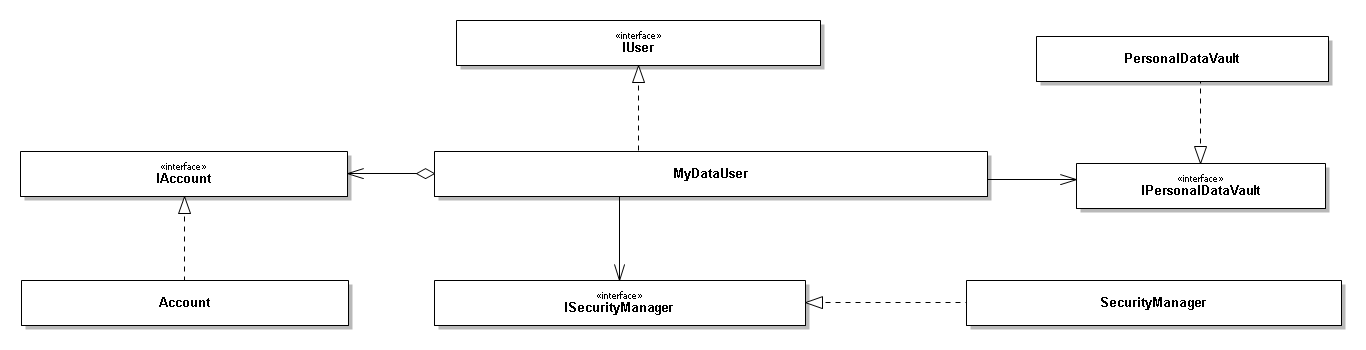
\includegraphics[width=\linewidth]{pictures/Accounting-closed.png}
	\caption{Diagramma UML delle classi di gestione degli account}
	\label{fig:Accounting-closed}
\end{figure}
Osservando il diagramma UML in figura \ref{fig:Accounting-closed} si osserva al centro la classe corrispondente all’utente \textit{MyData} che, confermando quanto detto in Analisi, \`e collegata agli account dei servizi e al \texttt{PersonalDataVault} dell’utente. Una novit\`a \`e invece rappresentata dalla coppia \texttt{ISecurityManager}, \texttt{SecurityManager} creata per soddisfare i requisiti di sicurezza relativi alla mutua autenticazione fra utente e servizio. Si \`e deciso di sviluppare separatamente questa classe per un principio di separazione delle responsabilit\`a e per consentire una estendibilit\`a pi\`u semplice in caso di sviluppi futuri.

\subsection{IUser, MyDataUser}
\begin{figure} [h]
	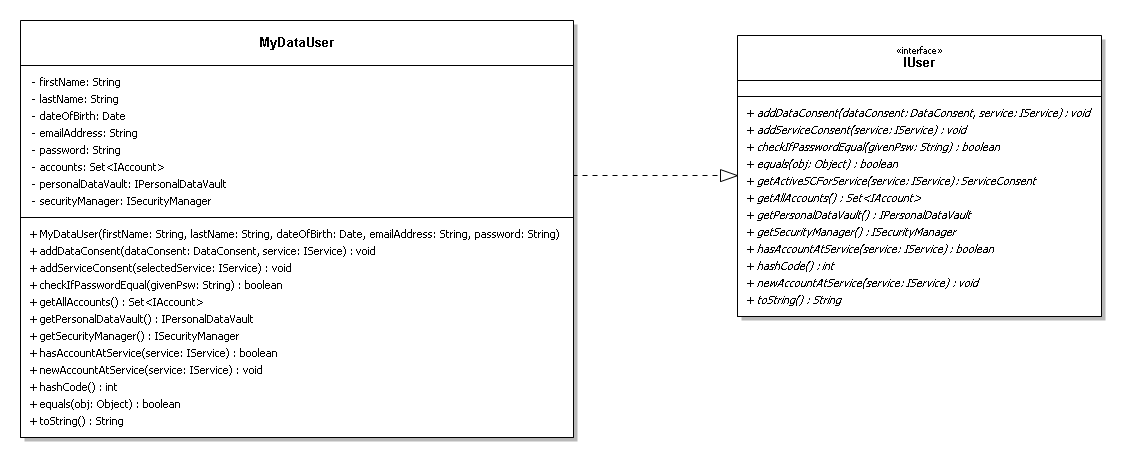
\includegraphics[width=\linewidth]{pictures/Accounting-MyDataUsr.png}
	\caption{Diagramma UML dell'implementazione di un account MyData}
	\label{fig:Accounting-MyDatUsr}
\end{figure}
Questa classe modella un generico utente dell’architettura \textit{MyData}. I field al suo interno sono un esempio delle caratteristiche che si \`e scelto di modellare e fra essi i pi\`u rilevanti sono indirizzo email e password in quanto permettono il login per utenti gi\`a registrati. L’indirizzo mail \`e stato adottato, inoltre, come identificatore unico di un utente all’interno di \textit{MyData} e questa caratteristica \`e stata implementata mediante l’override della funzione \texttt{equals(Object obj)}.

Si evidenzia inoltre la presenza di un \texttt{Set<IAccount> accounts} che realizza l’associazione fra un utente e gli account presso i servizi a cui si \`e registrato. La scelta di un \texttt{Set} permette di implementare il vincolo secondo cui ogni utente pu\`o avere un solo account presso un certo servizio ed \`e efficace anche perch\'e \`e superfluo mantenere un insieme ordinato di account.

Questa classe, inoltre, ha la funzione di interfacciare gli altri componenti del gestore, compresa la GUI, con gli account utente. A tal fine presenta i metodi \texttt{addServiceConsent (IService service)}, \texttt{addDataConsent (DataConsent dataConsent, IService service)}, \texttt{hasAccountAtService (IService service)}.  La classe \texttt{Account}, infatti, \`e stata modellata con visibilit\`a package protected per impedire l’accesso a classi esterne al package \texttt{users}: di conseguenza, anche la creazione di nuovi account avviene attraverso questa classe, in particolare nella funzione \texttt{newAccountAtService (IService service)}. All’interno del metodo troviamo l’istanziazione di un nuovo account insieme ad una chiamata alla classe \texttt{ConsentManager} che realizza quanto anticipato al paragrafo \ref{subsec:A-Consent}. In questo modo si ottiene un esempio di \textit{Service Linking} e l’esito di questa operazione viene concretizzato in un oggetto \texttt{ServiceConsent}. Si rimandano per\`o ulteriori dettagli a quanto evidenziato nella sezione \ref{sec:P-AutorizzazioniEConsent}.

\subsection{IAccount, Account}
\label{subsec:P-Account}
\begin{figure} [h]
	\centering
	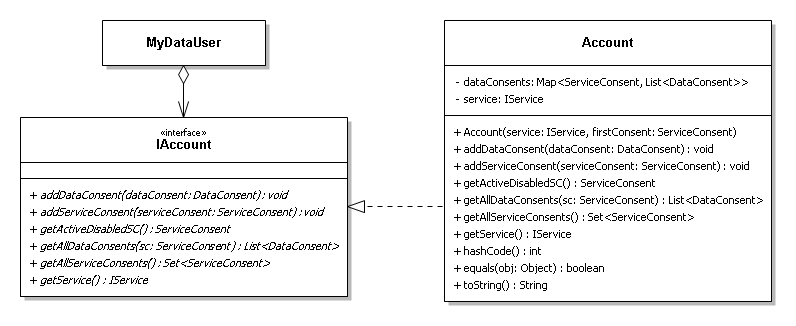
\includegraphics[width=0.95\linewidth]{pictures/Accounting-Account.png}
	\caption{Diagramma UML dell'implementazione di un account presso un servizio}
	\label{fig:Accounting-Account}
\end{figure}
La classe \texttt{Account} \`e abbastanza semplice poich\'e si occupa semplicemente di implementare la logica di basso livello nelle operazioni di gestione degli account.

Fra queste vi sono i controlli sullo stato dei \textit{Consent} memorizzati, la gestione dello storico di tutti i \textit{Consent} emessi per quel servizio \texttt{service} o ancora il matching fra i due tipi di \textit{Consent} (\texttt{ServiceConsent}, \texttt{DataConsent}, dettagliati al paragrafo \ref{subsec:P-ServiceConsentDataConsent} a pagina \pageref{subsec:P-ServiceConsentDataConsent}).

La memorizzazione dei \textit{Consent} all’interno della classe \`e stata ottenuta mediante l’utilizzo combinato delle strutture dati \texttt{Map<ServiceConsent, \-List\-<Data\-Consent>{}>}. Questa modalit\`a permette di esprimere diversi concetti a livello semantico. Innanzitutto per i \textit{Consent} sul flusso di dati si \`e scelto di utilizzare la classe base \texttt{DataConsent} invece che le sue due implementazioni, in modo da poterli memorizzare indiscriminatamente. Ci\`o verifica l’utilizzo del principio di sostituibilit\`a di Liskov. Inoltre, la scelta di una \texttt{List} come value all’interno di una mappa permette di descrivere un flusso di dati (all’interno dello stesso \texttt{ServiceConsent}) per il quale si sono rivelate necessare una molteplicit\`a di interazioni fra \textit{Source} e \textit{Sink}, ognuna delle quali modellata da un \texttt{DataConsent}.

Ad ogni istanza di \texttt{ServiceConsent} corrisponde quindi una \texttt{Collection} dei \texttt{DataConsent} emessi durante il periodo di validit\`a dello stesso ed \`e possibile avere un unico \texttt{ServiceConsent} attivo in un determinato istante di tempo.

\section{Servizi}
\label{sec:P-Service}
\begin{figure} [h]
	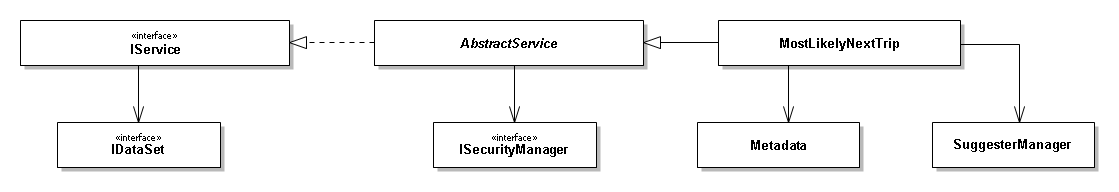
\includegraphics[width=\linewidth]{pictures/Services-closed.png}
	\caption{Diagramma UML per la rappresentazione di un servizio e delle sue dipendenze}
	\label{fig:Services-closed}
\end{figure}
Il diagramma UML in figura \ref{fig:Services-closed} mostra l’implementazione proposta per l’utilizzo di servizi all’interno dell’architettura \textit{MyData}. L’interfaccia \texttt{IService} e la classe astratta \texttt{AbstractService} sono state realizzate al fine di mediare l’interazione fra servizio concreto (in questo caso \textit{Most Likely Next Trip}) e Operatore (ad esempio, classi \texttt{ServiceRegistry} o \texttt{IMyData}). In questo senso, si pu\`o dire che la classe \texttt{AbstractService} raccoglie a fattore comune le operazioni comuni a tutti i servizi, lasciando alle classi figlie il compito di realizzare solo le parti fortemente dipendenti dalla particolare business logic. Per realizzare un nuovo servizio \`e necessario quindi creare una classe che estende \texttt{AbstractService}: nel caso di studio, essa \`e la classe \texttt{MostLikelyNextTrip} che si interfaccia con il servizio di calcolo del prossimo viaggio pi\`u probabile \cite{MLNT} \texttt{SuggesterManager}.

\subsection{IService, AbstractService, MostLikelyNextTrip}
\begin{figure} [h]
	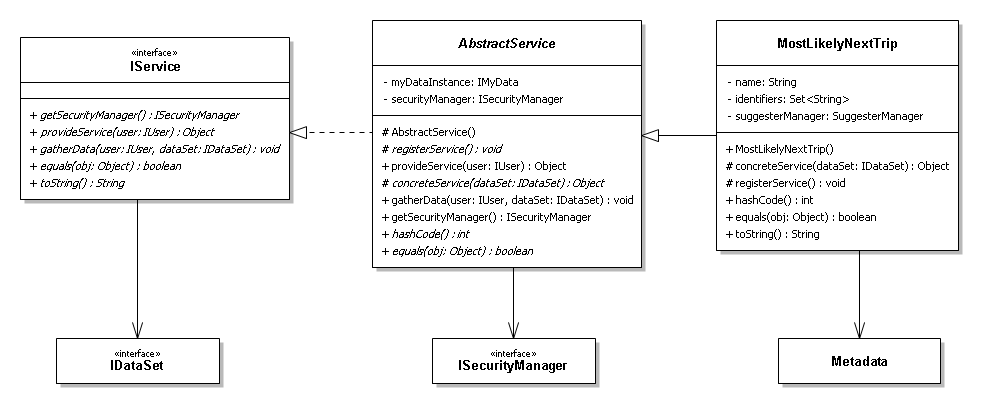
\includegraphics[width=\linewidth]{pictures/Services-open.png}
	\caption{Diagramma UML dell'implementazione di un servizio generico}
	\label{fig:Services-open}
\end{figure}
Il livello pi\`u astratto di definizione dei servizi in \textit{MyData} \`e rappresentato dall’interfaccia \texttt{IService}, e permette il loro riferimento all’interno dell’architettura. Fra i metodi esposti si evidenziano \texttt{provideService (IUser user)} e \texttt{gatherData (IUser user, dataSet IDataSet)}, che costituiscono i punti di ingresso e di uscita del flusso di dati utilizzati e prodotti dal servizio.

L’interfaccia viene implementata parzialmente dalla classe \texttt{AbstractService}. 

Il metodo \texttt{provideService} raccoglie a fattore comune la richiesta di un \texttt{OutputDataConsent} al \texttt{ConsentManager}, seguita dall’effettiva richiesta di dati inoltrata al \texttt{PersonalDataVault} tramite una richiesta alla classe \texttt{MyData}. Infine, viene restituito il risultato della chiamata alla funzione \texttt{abstract protected concreteService (IDataSet dataSet)}: la visibilit\`a garantisce che dall’esterno venga chiamato solo il metodo esposto dall’interfaccia \texttt{IService}. La signature astratta obbliga la ridefinizione del metodo nella classe figlia, che conterr\`a l'effettiva \textit{business logic} del servizio.

Il metodo \texttt{gatherData} segue la stessa sequenza di passi: la richiesta al \texttt{ConsentManager} di un \texttt{InputDataConsent} e l’interazione con il \texttt{PersonalDataVault} mediante Operatore \textit{MyData} sono per\`o preceduti da alcuni controlli sui dati in ingresso, al fine di verificare la legittimit\`a della richiesta.

Fra i metodi astratti si evidenzia infine \texttt{registerService()}, da invocare all’interno del costruttore della classe figlia. Durante la chiamata a procedura, il servizio concreto specifica quali tipi di dato utilizzer\`a mediante l’utilizzo delle costanti descritte in dettaglio nella sezione \ref{subsec:P-metadata}.

Della classe implementativa \texttt{MostLikelyNextTrip} si evidenzia solo la presenza dello stato interno, dove sono contenuti il nome, identificatore unico del servizio, e il \texttt{Set<String>} che contiene i tipi di dato utilizzati dal servizio.

\section{Operatore MyData}
Come previsto in fase di Analisi (sezione \ref{sec:A-mydataop}), si \`e proceduto alla realizzazione dell'Operatore \textit{MyData} tramite separazione delle responsabilit\`a, ottenendo come risultato le classi presentate nelle sottosezioni seguenti.

La sottosezione \ref{subsec:P-imydataMyData} presenta il nodo centrale del gestore di dati personali, che si occupa del coordinamento fra servizi, utente e Personal Data Storage. Svolge, insieme al \texttt{ConsentManager} (realizzato nella sottosezione \ref{subsec:P-CMConsStatus}), la funzione di \textit{policy enforcement}.

La sottosezione \ref{subsec:P-SecMan} presenta il componente \texttt{SecurityManager}, esempio di gestore delle politiche di sicurezza all'interno del progetto.

Infine, la sottosezione \ref{subsec:P-serviceregistry} presenta l'implementazione del \textit{Service Registry}.

\subsection{IMyData, MyData}
\label{subsec:P-imydataMyData}
\begin{figure} [h]
	\centering
	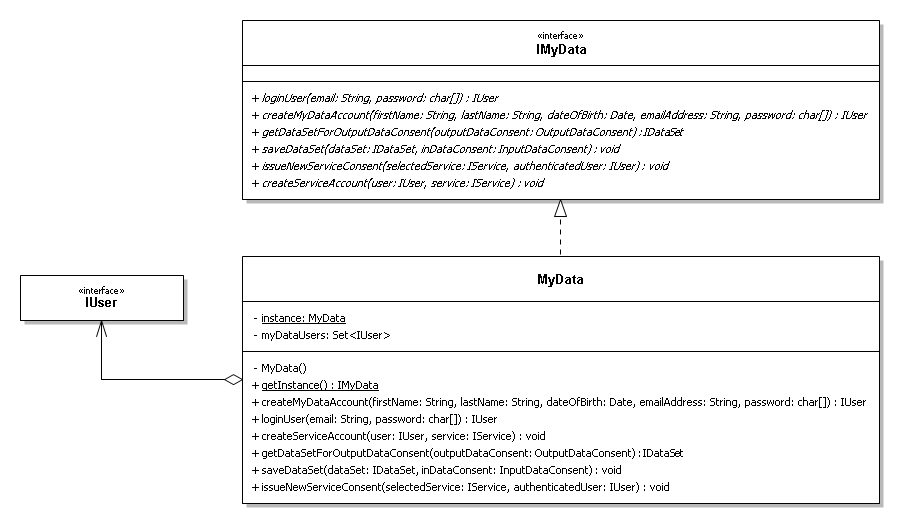
\includegraphics[width=0.8\linewidth]{pictures/MyData.png}
	\caption{Diagramma UML dell'implementazione di parte dell'Operatore MyData}
	\label{fig:Accounting-MyData}
\end{figure}
La classe \texttt{MyData} svolge all’interno del gestore di dati personali un importante ruolo di coordinamento fra le parti poich\'e realizza al suo interno una parte dell’Operatore \textit{MyData}, secondo quanto specificato in \ref{sec:A-mydataop}. Essa \`e il punto di riferimento per l’interfaccia utente a cui fornisce i dati da elaborare e mostrare a video e dalla quale riceve le richieste effettuate dall’utente.

Innanzitutto, si occupa di registrare e autenticare gli utenti (metodi \texttt{createMyDataAccount} e \texttt{loginUser}) in modo da impedire la creazione di duplicati. I controlli in questo senso vengono effettuati su un \texttt{HashSet<IUser>} contenuto all’interno della classe (si sfrutta la propriet\`a della struttura dati \texttt{Set} di non ammettere duplicati). La creazione di un nuovo account presso un determinato servizio viene gestita da questa classe tramite invocazione dell’opportuno metodo esposto dall’interfaccia \texttt{IUser}, insieme alla richiesta di nuovi \texttt{ServiceConsent} in caso di utente gi\`a registrato.

In secondo luogo, ogni servizio che ha richiesto e ottenuto il permesso di accedere a uno specifico insieme di dati personali di un utente fa riferimento alla classe \texttt{MyData}, che inoltra al Personal Data Vault quanto richiesto. L’operazione si svolge sia per i dati in ingresso che per i dati in uscita dal Vault mediante i metodi \texttt{getDataSetForOutputDataConsent (OutputDataConsent outputDataConsent)} e \texttt{saveDataSet (IDataSet dataSet, InputDataConsent inDataConsent)}. In entrambi i casi, viene controllata la validit\`a del \textit{Consent} emesso prima di effettuare la richiesta di dati personali.

Si evidenzia, infine, la realizzazione della classe \texttt{MyData} come Singleton mediante l’utilizzo di un costruttore privato e di un campo \texttt{instance} di tipo \texttt{MyData}. Ci\`o assicura la presenza di un unico Operatore di questo tipo all’interno del programma.

\subsection{SecurityManager}
\label{subsec:P-SecMan}
\begin{figure} [h]
	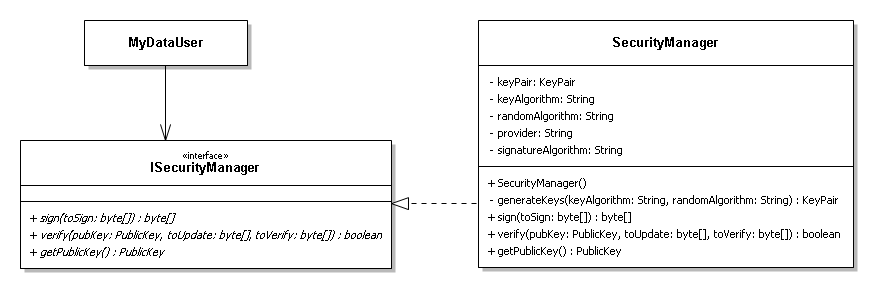
\includegraphics[width=\linewidth]{pictures/Accounting-SecurityManager.png}
	\caption{Diagramma UML del gestore delle operazioni di sicurezza}
	\label{fig:Accounting-SecurityManager}
\end{figure}
Come anticipato nella sezione \ref{sec:P-accounting}, si \`e resa necessaria l'implementazione di un'entit\`a che garantisse il rispetto di alcune politiche di sicurezza.

In particolare, in questa implementazione si \`e scelto di dare maggiore rilevanza all'aspetto di reciproca autenticazione fra utente e servizio, piuttosto che ad altre problematiche quali ad esempio memorizzazione e trasmissione sicura dei dati. A tal fine si \`e scelto di utilizzare alcuni componenti gi\`a pronti all'interno dell'infrastruttura Java, in particolare all'interno della Java Cryptography Architecture \cite{javacrypto}.

Per realizzare un protocollo di sfida e risposta, la classe \texttt{SecurityManager} contiene una coppia di chiavi \texttt{KeyPair}, insieme ad alcune costanti che rappresentano gli algoritmi ed il provider scelto per l'implementazione degli stessi.

L'interfaccia \texttt{ISecurityManager} ha la funzione di astrarre dalla particolare implementazione (ogni servizio potrebbe ad esempio preferire una implementazione specifica), e pertanto espone solamente i metodi di firma e verifica necessari al completamento dell'operazione di autenticazione.

\subsection{ServiceRegistry}
\label{subsec:P-serviceregistry}
\begin{figure} [h]
	\centering
	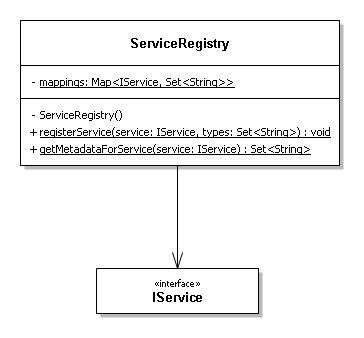
\includegraphics[width=0.5\linewidth]{pictures/ServiceRegistry.png}
	\caption{Diagramma UML dell'implementazione del Service Registry}
	\label{fig:ServiceRegistry}
\end{figure}
Ogni servizio che voglia essere utilizzabile all’interno dell’infrastruttura \textit{MyData} deve innanzitutto registrarsi all’interno del \textit{Service Registry}. In fase di registrazione, ogni servizio dichiara quali siano i tipi di dato necessari per il suo funzionamento, al fine di agevolare gli scambi di dati con altre entit\`a dell’infrastruttura, siano esse \textit{Source} o \textit{Sink}.

Per questo motivo, la classe \texttt{ServiceRegistry} ha come responsabilit\`a fondamentale quella di mantenere al suo interno le corrispondenze fra i servizi registrati e i tipi di dato: ci\`o viene realizzato mediante l’utilizzo di una \texttt{Map<IService, Set<String>{}>}.

Come per la classe \texttt{ConsentManager} (analizzata pi\`u in dettaglio nella sottosezione \ref{subsec:P-CMConsStatus}), anche in questo caso si \`e cercato di rendere il \textit{Service Registry} il pi\`u possibile indipendente tramite l’uso di metodi statici e la scelta di un costruttore privato. I metodi \texttt{registerService(IService service, Set<String> types)} e \texttt{Set<String> getMetadataForService(IService service)} incapsulano quelli di basso livello esposti dalla struttura dati \texttt{Map}, aggiungendo opportuni controlli sui parametri in ingresso. In particolare, \`e possibile registrare un servizio mediante la procedura \texttt{registerService} e ottenere i tipi di dato registrati mediante la funzione \texttt{getMetadataForService}.

\section{Autorizzazioni e Consent}
\label{sec:P-AutorizzazioniEConsent}
\begin{figure} [h]
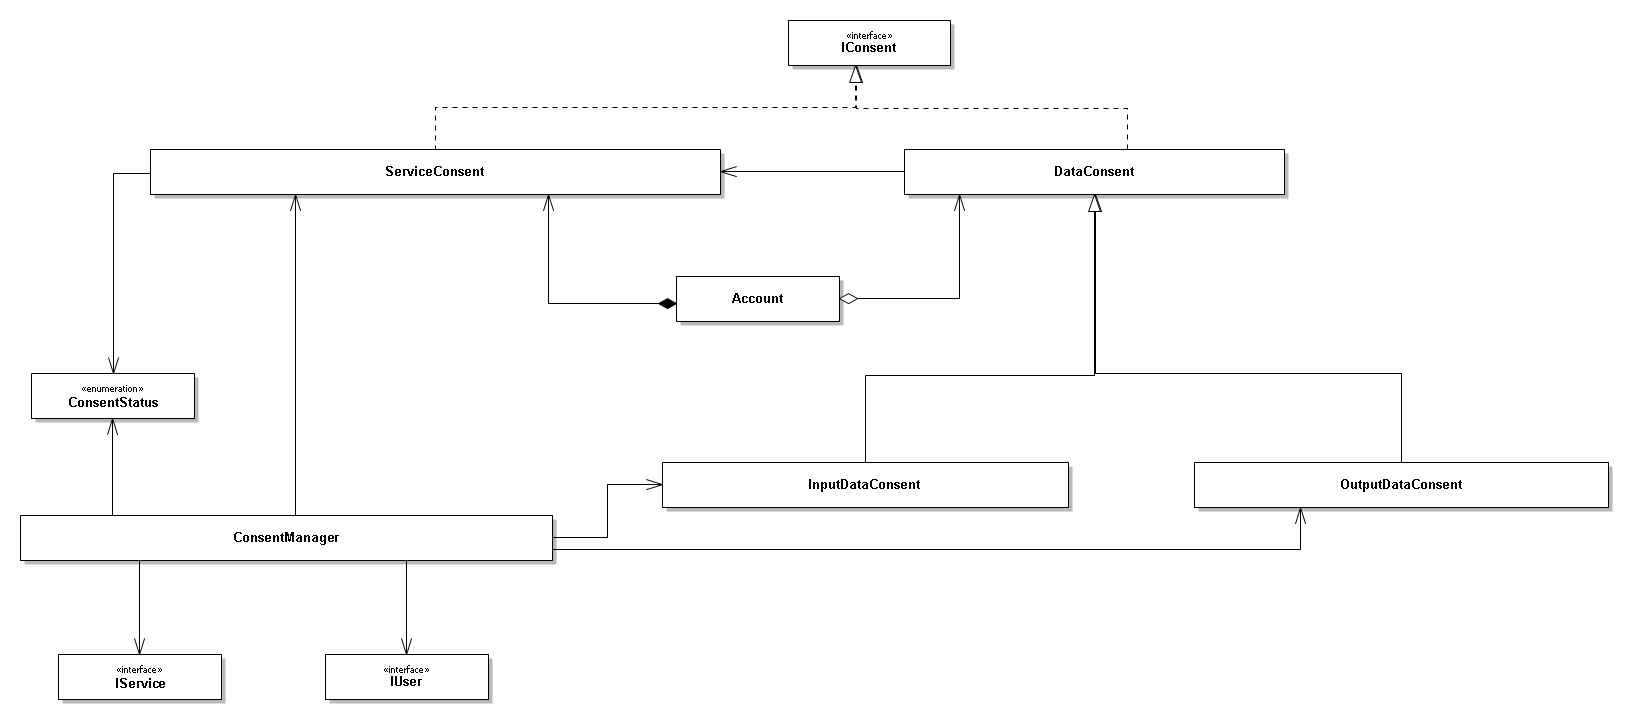
\includegraphics[width=\linewidth]{pictures/Auth-closed.png}
\caption{Diagramma UML dell'architettura per la gestione dei permessi}
\label{fig:Auth-closed}
\end{figure}
All'interno dell'architettura realizzata per la gestione delle autorizzazioni e dei permessi \`e possibile individuare alcune entit\`a fondamentali: la classe \texttt{ConsentManager}, che realizza il gestore di permessi previsto nella sezione \ref{sec:A-mydataop}, e le due tipologie di permessi, anch’esse previste in fase di Analisi (sottosezione \ref{subsec:A-Consent}).

\`E presente, infine, anche l’enumerativo \texttt{ConsentStatus} attraverso il quale si rappresentano gli stati del rapporto fra un utente ed un servizio generici.

\subsection{ConsentManager, ConsentStatus}
\label{subsec:P-CMConsStatus}
\begin{figure} [h]
	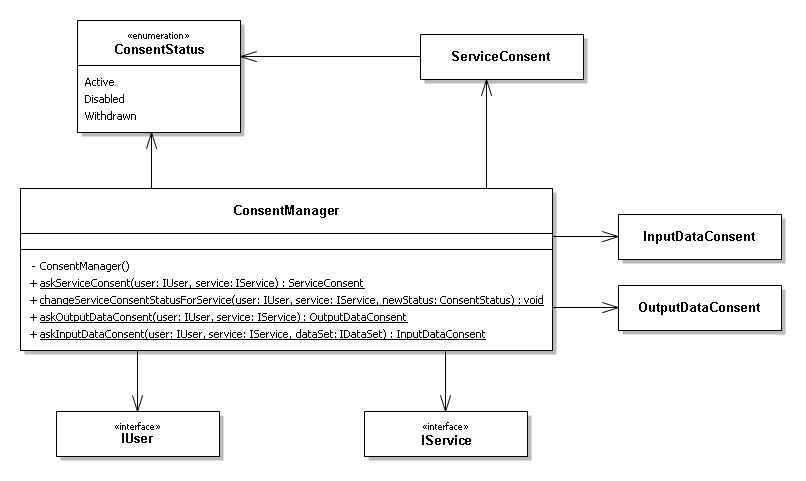
\includegraphics[width=\linewidth]{pictures/Auth-CM.png}
	\caption{Diagramma UML del gestore di permessi}
	\label{fig:Auth-CM}
\end{figure}
La classe \texttt{ConsentManager} si occupa dell’erogazione, in caso di richiesta legittima, di vari tipi di permessi ai servizi che ne fanno richiesta. Poich\'e il suo scopo \`e quello di garantire il rispetto di un determinato protocollo di assegnazione dei permessi, essa \`e innanzitutto una classe implementativa e pertanto motivo non \`e previsto alcun tipo di astrazione (ad esempio tramite interfaccia).

Si potrebbe considerare di rendere la classe \texttt{final} per impedire estensioni o ridefinizioni del comportamento. Le motivazioni a supporto di questa scelta risiedono nella garanzia di una maggiore sicurezza. Nel complesso, tuttavia, ci\`o porterebbe ad una eccessiva rigidit\`a del codice, impedendo aggiornamenti del protocollo anche in casi di legittima necessit\`a.

Si \`e cercato di realizzare un servizio il pi\`u possibile indipendente dall'architettura circostante: pertanto, la classe \texttt{ConsentManager} non mantiene alcuno stato interno, presenta costruttore privato e non ha dipendenze rilevanti. Inoltre, poich\'e la procedura di verifica dei requisiti \`e costante e indipendente dai parametri di ingresso, ogni metodo \`e stato realizzato come \texttt{static}. 

I tipi di \textit{Consent} erogati dalla classe \texttt{ConsentManager} sono \texttt{ServiceConsent}, \texttt{InputDataConsent} e \texttt{OutputDataConsent}, ognuno con un metodo dedicato. \`E presente anche la procedura \texttt{changeServiceConsentStatusForService (IUser user, IService service, ConsentStatus newStatus)}, che permette all’utente di cambiare lo stato del \texttt{ServiceConsent} correntemente attivo o disabilitato, secondo quanto previsto dalle specifiche di \textit{MyData} e successivamente in fase di Analisi (sottosezione \ref{subsec:A-Consent}).

\subsection{ServiceConsent, DataConsent}
\label{subsec:P-ServiceConsentDataConsent}
\begin{figure} [h]
	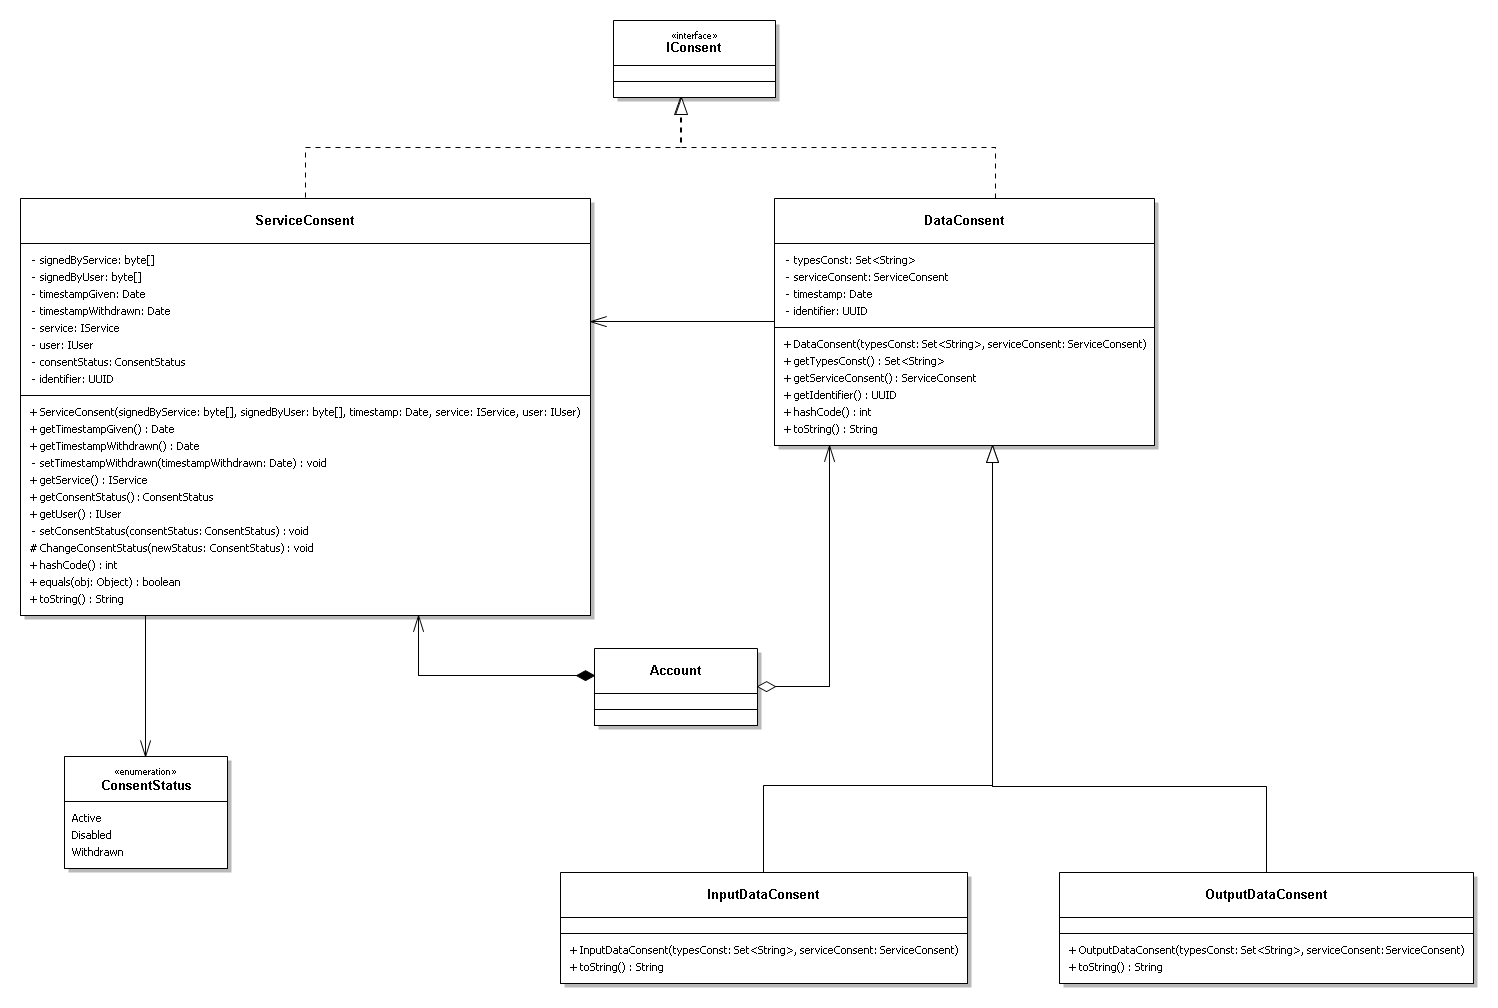
\includegraphics[width=\linewidth]{pictures/Auth-Consents.png}
	\caption{Diagramma UML dei due tipi di permessi e delle loro dipendenze}
	\label{fig:Auth-Consents}
\end{figure}
I permessi utilizzati all’interno del gestore di dati personali ed erogati dalla classe \texttt{ConsentManager} sono istanze delle classi \texttt{ServiceConsent}, \texttt{InputDataConsent} e \texttt{OutputDataConsent}. Come \`e possibile osservare dal diagramma UML in figura \ref{fig:Auth-Consents}, \texttt{InputDataConsent} e \texttt{OutputDataConsent} estendono la classe \texttt{DataConsent}: la loro funzione \`e principalmente semantica, poich\'e non aggiungono logica al programma ma descrivono il verso del flusso di dati che si crea con il Personal Data Vault. Pertanto, descriver\`o principalmente le caratteristiche delle classi \texttt{ServiceConsent} e \texttt{DataConsent} che costituiscono il punto focale della realizzazione dei permessi descritti in \textit{MyData}.

Nonostante la differenza di realizzazione e di utilizzo, entrambe le classi \texttt{ServiceConsent} e \texttt{DataConsent} implementano una interfaccia comune \texttt{IConsent}. Questa \`e una interfaccia \textit{marker} necessaria per esprimere una somiglianza a livello semantico, in quanto entrambe le classi descrivono un tipo di autorizzazione.

Dal diagramma UML \`e possibile dedurre il ruolo della classe \texttt{Account} rispetto ai due tipi di \textit{Consent}. Come accennato infatti in \ref{subsec:P-Account}, essa mantiene al suo interno una mappa di corrispondenze fra \texttt{ServiceConsent} e liste di \texttt{DataConsent}.

Nel primo caso, la relazione \`e rappresentata mediante il simbolo “rombo nero” che qualifica la classe \texttt{Account} come “contenitore” di istanze della classe \texttt{ServiceConsent}. In particolare, il rombo nero descrive un tipo di relazione molto stretta fra le due parti e la scelta \`e dovuta alle specifiche di \textit{MyData}, secondo cui non \`e possibile registrarsi presso un servizio senza ottenere un \textit{Consent}. Ci\`o \`e stato implementato mediante l’emissione di un \texttt{ServiceConsent} prima della creazione effettiva dell’account e il legame fra i due avviene tramite il passaggio di questo permesso al costruttore della classe \texttt{Account}.

La classe \texttt{ServiceConsent} realizza il primo – e il pi\`u rilevante – dei due tipi di permessi previsti per il gestore di dati personali. Al suo interno troviamo i \textit{token} firmati da utente e servizio per la mutua autenticazione, insieme ai rispettivi riferimenti; vi sono, inoltre, anche alcuni campi per l’identificazione del \textit{Consent} stesso e la sua collocazione temporale.

Per quanto riguarda invece i \texttt{DataConsent}, essi si comportano come \textit{access token} per il Personal Data Vault, sono validi una sola volta e vengono conservati come storico dell’accesso ai dati personali. A tal fine, un \texttt{DataConsent} contiene al suo interno il \texttt{Set<String>} con l’elenco dei tipi di dato a cui il servizio beneficiario pu\`o accedere. Per impedire accessi illegittimi, viene sempre controllata la corrispondenza fra i tipi di dato dichiarati in fase di registrazione e quelli richiesti alla creazione del \texttt{DataConsent}. Poich\'e il servizio non pu\`o interrogare direttamente il Personal Data Vault, gli scambi avvengono in base a quanto dichiarato all’interno del \texttt{Set<String>}.

Dal diagramma UML, infine, viene evidenziato che ogni \texttt{DataConsent} mantiene un riferimento al \texttt{ServiceConsent} attivo al momento della sua emissione, al fine di ottenere una migliore tracciabilit\`a delle transazioni di dati e che il costruttore della stessa classe ha visibilit\`a package - protected in modo da obbligare l’uso delle sottoclassi alle classi esterne.

\section{Rappresentazione e gestione dei dati personali}
\label{sec:P-datinonnotiapriori}
Si presenta a questo punto la problematica di rappresentazione dei dati, non solo all’interno del Personal Data Storage ma anche durante le transazioni fra \textit{Source} e \textit{Sink} e all’interno del servizio stesso.

La soluzione implementata all’interno del Mobility Profile prevede l’uso di oggetti JsonArray e GeoJSON, come indicato nella documentazione  \cite{githubmobilityprofilespecification}, tuttavia questa implementazione differisce dal caso di studio poich\'e il servizio che utilizza i dati per calcolare il prossimo viaggio pi\`u probabile e il Personal Data Storage si trovano all’interno della stessa app. Come evidenziato in \ref{sec:Contesto-MobProfJPlann} infatti, l’applicazione Journey Planner \`e solamente un frontend che non esegue alcuna computazione ma presenta un risultato gi\`a pronto.

All’interno del gestore di dati personali in oggetto si vuole invece permettere un flusso di dati fra \textit{Source} e \textit{Sink} generici in modo che la computazione avvenga presso il servizio che richiede i dati e non localmente al Personal Data Storage.

Tale problema \`e stato rappresentato in fase di Analisi (sezione \ref{sec:A-datinonnotiapriori}) e si \`e proposta come soluzione l’utilizzo del formato JSON per la comunicazione e il trasferimento di dati.

In questo contesto, si sono valutati innanzitutto i componenti Java disponibili nell’architettura per realizzare la conversione in stringhe JSON: \texttt{JsonArray}, \texttt{JsonObject} e altre sotto-interfacce di \texttt{JsonValue} \cite{java8api}. Non si \`e ritenuto di doverli utilizzare perch\'e questi non offrono alcun metodo di utilit\`a per la conversione da oggetto a stringa e la trasposizione di ogni \textit{field} va realizzata manualmente sia in serializzazione che in deserializzazione. Una scelta di questo tipo implicherebbe un precedente accordo fra le parti per stabilire come interpretare le stringhe inviate e una forte dipendenza dalla particolare implementazione delle classi.

Come seconda opzione si \`e considerato di utilizzare la libreria Google Gson \cite{googlegson}, in quanto risolve i problemi incontrati nel corso del primo tentativo grazie ai metodi \texttt{gson.toJson(obj)} per la serializzazione e \texttt{gson.fromJson\-(json,\- obj.class)} per la deserializzazione. Questo approccio, che funziona perfettamente in caso di oggetti che contengono tipi primitivi, mostra qualche limitazione quando si introducono oggetti di tipo generico e \texttt{Collection} di oggetti, siano esse di oggetti di un unico tipo o di tipi diversi. Il motivo risiede nell’implementazione della Java Virtual Machine e, in particolare, nella sua caratteristica di \textit{Type Erasure} per la quale ogni oggetto a basso livello “perde” il suo tipo particolare per diventare un \texttt{Object}. Ci\`o non crea problemi in serializzazione ma pu\`o crearli in deserializzazione, quando risulta impossibile recuperare il tipo originario dell’oggetto da deserializzare. Poich\'e l’utilizzo della libreria Gson nel contesto del \texttt{PersonalDataVault} si sarebbe collocato all’interno dei casi non completamente supportati, si \`e scelto di scartare anche questa seconda possibilit\`a.

Tale problematica (impossibilit\`a di prevedere con sufficiente precisione tutte le possibili situazioni legate alla rappresentazione dei dati in ogni momento) riveste un serio aspetto di complessit\`a e articolazione da assumere una rilevanza non contenibile nei limiti del presente lavoro di tesi.

Necessiterebbe, viceversa, di organizzazione, mezzi e tempistiche - oltre che conoscenze - non immediatamente disponibili nell'attuale contesto. Si rende necessario, pertanto, ricercare una soluzione diversa, pi\`u concreta e adeguata alle attuali circostanze e pi\`u ammissibile anche rispetto agli obiettivi di questo lavoro.

L'ipotesi che viene proposta e che pu\`o ritenersi pi\`u accettabile, consiste nell’utilizzo di una struttura dati \texttt{DataSet} che permetta lo scambio di dati di qualunque tipo all’interno del sistema, purch\'e il loro tipo sia stato preventivamente dichiarato in fase di registrazione (sottosezione \ref{subsec:P-serviceregistry}). La classe \texttt{DataSet} viene descritta in dettaglio nella sottosezione \ref{subsec:P-metadata}.

\subsection{Memorizzazione: PersonalDataVault}
\label{subsec:P-PDV}
\begin{figure} [h]
	\centering
	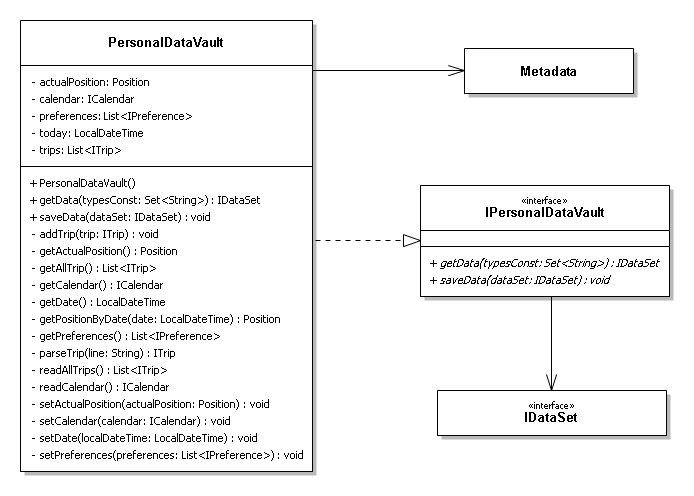
\includegraphics[width=0.8\linewidth]{pictures/PersonalDataVault.png}
	\caption{Diagramma UML dell'implementazione di un Personal Data Storage}
	\label{fig:PersonalDataVault}
\end{figure}
In questa sezione si presenta la classe \texttt{PersonalDataVault}, in cui vengono mantenuti i dati personali dell’utente. Essa corrisponde direttamente al Personal Data Storage proposto all’interno della documentazione \textit{MyData}.

L’interfaccia \texttt{IPersonalDataVault} espone i metodi \texttt{getData (Set<String> typesConst)} (che restituisce un \texttt{IDataSet}) e \texttt{saveData (IDataSet dataSet)} che permettono l’accesso ai dati. Essi si occupano di prelevare dati, o salvarli, in base a quanto specificato dal \texttt{Set<String>} contenente l’insieme dei tipi di dato. Inoltre, la signature garantisce l’indipendenza dai tipi di dato in ingresso o in uscita dal Vault grazie all’uso di oggetti di tipo \texttt{DataSet} incapsulati in opportune interfacce \texttt{IDataSet}. 

All’interno della classe \texttt{PersonalDataVault} troviamo alcuni metodi privati necessari per la gestione dei dati memorizzati (ad esempio la lettura e la scrittura su file, con opportune funzioni di utility necessarie per il parsing). Le scelte effettuate in questo senso derivano da una precedente implementazione e sono state adattate solo in minima parte per motivi di compatibilit\`a. Per quanto riguarda invece i metodi ereditati dall’interfaccia, si evidenzia l’eventualit\`a di una \texttt{RuntimeException} (\texttt{ClassCastException}): il verificarsi di questo evento, pur non auspicabile, rappresenta comunque uno stato del sistema previsto e voluto. Qualora infatti un oggetto dovesse rivelarsi di un tipo diverso rispetto a quello dichiarato all’interno del \texttt{dataSet} ricevuto in ingresso, \`e opportuno che il programma segnali questa grave inconsistenza terminando la sua esecuzione. Incidentalmente, il verificarsi di una siffatta situazione implica la violazione delle politiche e dei protocolli di sicurezza e pertanto si ritiene motivato l’utilizzo di questa eccezione di basso livello.

Si pu\`o osservare che l’implementazione del \texttt{PersonalDataVault} \`e particolarmente dipendente dai tipi di dato utilizzati dal servizio \textit{Most Likely Next Trip} scelto come caso di studio. Tale caratteristica costituisce una limitazione del gestore di dati personali realizzato in questa tesi e trova un riscontro all’interno delle problematiche evidenziate all’interno della sezione \ref{sec:P-datinonnotiapriori}. Anche la scelta di memorizzare i dati acquisiti all’interno di file di testo, derivata da una precedente implementazione, si colloca all’interno di un orizzonte limitato: alcune proposte di aggiornamento sono state discusse in \ref{sec:A-PDS}, e saranno oggetto di ulteriore discussione all’interno del capitolo \ref{capitolo6}.

\subsection{Rappresentazione: Metadata}
\label{subsec:P-metadata}
\begin{figure} [h]
	\centering
	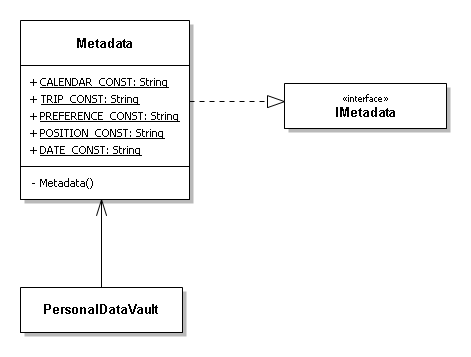
\includegraphics[width=0.7\linewidth]{pictures/Metadata.png}
	\caption{Diagramma UML della classe per la rappresentazione dei dati}
	\label{fig:Metadata}
\end{figure}
Come gi\`a accennato in precedenza, un approccio diverso, pi\`u completo ed esaustivo, avrebbe comportato mezzi pi\`u consistenti e conoscenze di cui - al momento - non si dispone.

Si \`e ritenuto, in alternativa, di dover ricorrere alla definizione preventiva dei tipi di dato disponibili all’interno del sistema, quali ad esempio \texttt{Position} e \texttt{ICalendar}, utilizzando, dove possibile, le interfacce al posto delle classi, onde diminuire la forte dipendenza dalla particolare implementazione.

Questa modalit\`a potrebbe forse apparire come una eccessiva semplificazione del contesto per la scelta arbitraria dei tipi di alto livello sopra menzionati e delle loro implementazioni. La soluzione proposta, per\`o, \`e da ritenersi plausibile in quanto valuta che i componenti indicati siano tali da poter rendere risultati accettabili anche in presenza delle limitazioni assunte.

Pertanto, la classe \texttt{Metadata} ha il compito di definire a priori i tipi di dato disponibili all’interno dell’Operatore \textit{MyData}. A livello implementativo, la classe espone un certo numero di stringhe \texttt{static final}, ognuna delle quali \`e inizializzata con il \textit{fully qualified name} della classe (o interfaccia) che rappresenta, al fine di conservare l’informazione completa riguardo al tipo di dato. All’interno del programma, esse sono accessibili mediante la notazione \texttt{Metadata.DATATYPE\_CONST}, ad esempio al momento della costruzione dei \texttt{Set<String>} necessari per la registrazione presso il \texttt{ServiceRegistry} (sottosezione \ref{subsec:P-serviceregistry}), o nel controllo della legittimit\`a dell’emissione di un permesso (sottosezione \ref{subsec:P-CMConsStatus}).

\subsection{Trasferimento: IDataSet}
\begin{figure} [h]
	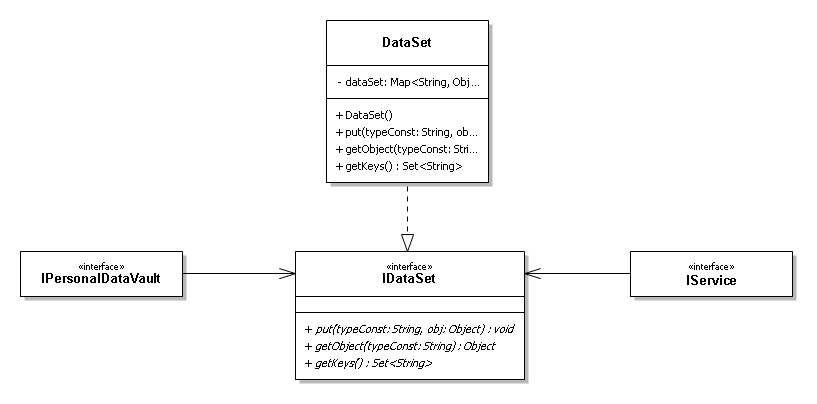
\includegraphics[width=\linewidth]{pictures/IDataSet.png}
	\caption{Diagramma UML della classe per il trasferimento dei dati}
	\label{fig:IDataSet}
\end{figure}
Come anticipato nelle sezioni precedenti, la classe \texttt{DataSet} viene utilizzata per il trasferimento di dati fra \textit{Source} e \textit{Sink}. Essa si riferisce e realizza il concetto di Resource Set Identifier, insieme alle oportune modifiche introdotte in fase di Analisi (sottosezione \ref{subsec:A-granularitaConsent}).
 Dal grafico UML in figura \ref{fig:IDataSet} si nota che essa viene sempre referenziata per mezzo dell’interfaccia \texttt{IDataSet}, ed \`e inoltre possibile riconoscere \texttt{IPersonalDataVault} e \texttt{IService} nei ruoli (non statici) di \textit{Source} e \textit{Sink}.

L’oggetto \texttt{DataSet} contiene i dati da trasferire mediante l’utilizzo di una \texttt{Map<String, Object>}, dove le chiavi sono le costanti di tipo stringa esposte dalla classe \texttt{Metadata} e i \textit{value} corrispondenti sono generici \texttt{Object} (non sono permessi valori \texttt{null}). In altre parole, questa struttura dati associa ad ogni oggetto il suo tipo, espresso all’interno di una stringa.

L’obiettivo della classe \texttt{DataSet} \`e contenere un insieme di oggetti potenzialmente diversi il cui tipo non \`e noto a priori, senza perdere l’informazione sul tipo stesso dopo la conversione a \texttt{Object}.

In questo modo si trova una soluzione al problema della \textit{Type Erasure}, poich\'e l’informazione sul tipo di dato originario viene conservata separatamente all’oggetto stesso. Il destinatario della trasmissione \`e in grado, attraverso le costanti di tipo stringa, di risalire al tipo dell’oggetto ricevuto, in modo da poterlo utilizzare in modo appropriato.

I metodi esposti dall’interfaccia ridefiniscono quelli propri della struttura dati \texttt{Map} che costituisce lo stato interno della classe, aggiungendo il controllo per i valori \texttt{null} e per la richiesta di oggetti non disponibili all’interno della mappa data.

\section{Uso delle eccezioni}
All’interno del gestore di dati personali sviluppato nell’ambito di questa tesi, \`e di importanza non trascurabile il controllo della legittimit\`a delle operazioni da eseguire, degli argomenti in ingresso alle funzioni o degli stati in cui si trova il gestore stesso. \`E necessario, pertanto, uno strumento che permetta di descrivere il verificarsi di situazioni non previste o illegittime, impedendo la continuazione del flusso del programma. Questa situazione \`e diversa, ad esempio, dal caso in cui l’invocazione di un metodo \`e legittima ma non produce alcuni risultato, poich\'e \`e di fondamentale importanza che l’esecuzione termini.

Lo strumento utilizzato per ottenere questa caratteristica sono le Java \texttt{Exception}, ed in particolare le sottoclassi di \texttt{RuntimeException} \texttt{IllegalArgumentException}, \texttt{IllegalStateException} e \texttt{SecurityException}. 

Fra di esse, \texttt{IllegalStateException} \`e descritta all’interno della documentazione Java nel modo seguente:
\begin{quote}
“Signals that a method has been invoked at an illegal or inappropriate time. In other words, the Java environment or Java application is not in an appropriate state for the requested operation” \cite{java8api}.
\end{quote}
Si \`e valutato quindi che questa eccezione fosse adeguata in tutti quei casi in cui l’invocazione di un metodo non pu\`o essere portata a termine a causa di \textit{Consent} non adeguati. Un esempio pu\`o essere la richiesta di un nuovo \texttt{DataConsent} nel caso in cui non vi sia un \texttt{ServiceConsent} attivo in quel momento.

L’uso di \texttt{IllegalArgumentException} \`e convenzionalmente limitato al controllo dei parametri in ingresso ai metodi, in aderenza a quanto dichiarato sulla documentazione Java. Fra le \texttt{RuntimeException} utilizzate \`e presente anche \texttt{SecurityException}, invocata ogni volta in cui un parametro o controllo di sicurezza non \`e verificato.

Un aspetto importante dell’uso delle eccezioni \`e stata la loro collocazione all’interno dello \textit{stack} delle invocazioni di metodi. Si prenda come esempio il caso di richiesta di un nuovo \texttt{DataConsent}: \`e noto a priori che la precondizione per ottenerlo richiede l’esistenza di un \texttt{ServiceConsent} attivo in quel momento. Questa eventualit\`a \`e controllata all’interno della classe \texttt{ConsentManager} mediante l’uso di una \texttt{IllegalStateException}. Tuttavia esiste un sotto-caso che, pur rientrando a pieno titolo nell’insieme di situazioni non corrette (mancanza di un \texttt{ServiceConsent} attivo), merita di essere differenziato per il suo valore semantico. Si tratta infatti del caso in cui l’utente per cui si avanza la richiesta non sia registrato presso il servizio: il \texttt{ServiceConsent} non ha stato \textit{Active} perch\'e in realt\`a non ne \`e stato emesso alcuno. Al fine di controllare anche questa eventualit\`a \`e opportuno inserire una eccezione nella classe \texttt{MyDataUser} invece che \texttt{ConsentManager}, in quanto ci\`o rientra all’interno del suo ambito di responsabilit\`a.

\section{Graphical User Interface}
Per la realizzazione dell’interfaccia grafica del gestore di dati personali si \`e scelto il design pattern Model View Controller. Questo viene impiegato anche all’interno di \textit{Most Likely Next Trip} \cite{MLNT}, del quale si \`e utilizzata la schermata di funzionamento del servizio omonimo.

Si \`e ritenuto necessaria, in questo contesto, la realizzazione di due finestre con le seguenti funzioni:
\begin{itemize}
	\item Una schermata per login e registrazione, realizzata in figura \ref{fig:welcomePanel};
	\item Una schermata per il profilo utente, che mostri i servizi attivi e abiliti, o disabiliti, determinati pulsanti a seconda dello stato corrente dell’esecuzione, mostrato in figura \ref{fig:exampleConsentInProj}.
\end{itemize}
\begin{figure} 
	\centering
	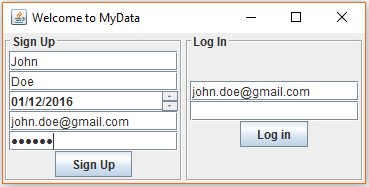
\includegraphics[width=0.5\linewidth]{pictures/welcomePanel.png}
	\caption{Schermata di login con esempio di registrazione al gestore di dati personali}
	\label{fig:welcomePanel}
\end{figure}
\begin{figure}
	\centering
	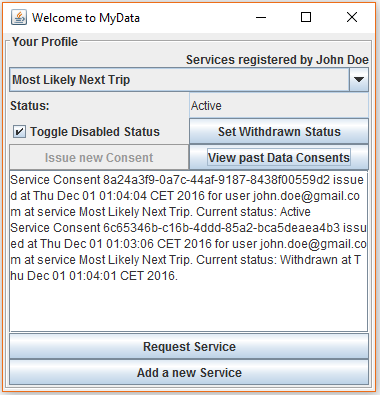
\includegraphics[width=0.5\linewidth]{pictures/exampleConsentInProj.png}
	\caption{Profilo utente con esempio di Consent Attivo e Ritirato}
	\label{fig:exampleConsentInProj}
\end{figure}
A ci\`o si deve aggiungere la schermata del servizio, che viene mostrata ad ogni sua invocazione (figura \ref{fig:MLNTPanel}).
\begin{figure}
	\centering
	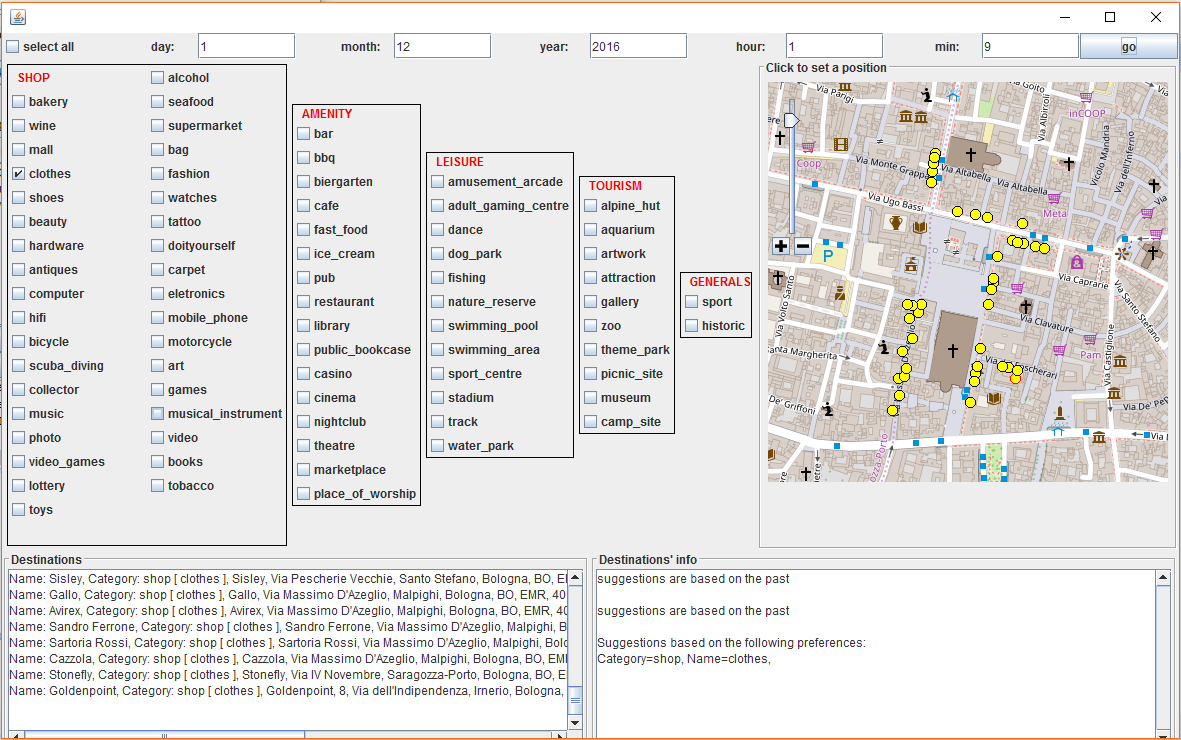
\includegraphics[width=0.85\linewidth]{pictures/MLNTPanel.png}
	\caption{Schermata di\textit{ Most Likely Next Trip} con esempio di invocazione}
	\label{fig:MLNTPanel}
\end{figure}

Il Controller ha lo scopo di gestire la View e di realizzare una comunicazione con il Model: per quest’ultimo aspetto, esso si interfaccia quasi unicamente con la classe \texttt{MyData}, confermando il suo ruolo centrale di gestione.

La View mostra il profilo dell’utente loggato, permettendo la gestione dei servizi a cui si \`e registrato. \`E possibile aggiungere nuovi servizi (funzione implementata tramite mock per mancanza di \textit{Service Linking}), visualizzare le autorizzazioni emesse modificare il loro stato.

Nella figura \ref{fig:exampleConsentInProj} vediamo il profilo utente: dal men\`u a tendina in alto \`e possibile scegliere un servizio all’interno di quelli registrati; subito sotto sono presenti alcuni comandi per la gestione del suo stato (\`e possibile impostare i valori \textit{Active}, \textit{Disabled}, \textit{Withdrawn}) e per l’emissione di nuove autorizzazioni in caso di necessit\`a. \`E presente inoltre una casella di testo in cui sono mostrati tutti i \texttt{ServiceConsent} relativi al servizio selezionato e tramite la pressione di un bottone si apre una nuova finestra che mostra i relativi \texttt{DataConsent} (figura \ref{fig:DataConsentFrame}). Infine, si trovano i bottoni per invocare il servizio e il \textit{Service Registry}.
\begin{figure}
	\centering
	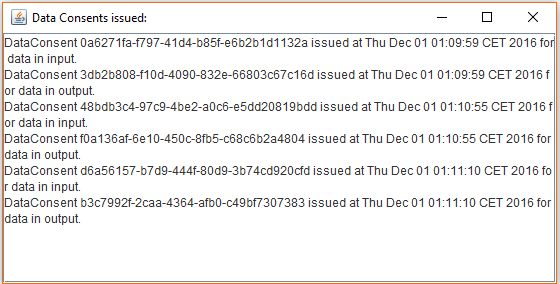
\includegraphics[width=0.5\linewidth]{pictures/DataConsentFrame.png}
	\caption{Esempio di flusso di permessi \texttt{DataConsent}}
	\label{fig:DataConsentFrame}
\end{figure}
	\chapter{Conclusioni e sviluppi futuri}
\label{capitolo6}
\thispagestyle{empty}

\noindent placeholder.

	\clearpage{\pagestyle{empty}\cleardoublepage}
	%\addcontentsline{toc}{chapter}{Bibliografia}
	\bibliographystyle{plain}
	\bibliography{bibl_tesi}

	\clearpage{\pagestyle{empty}\cleardoublepage}	
	\chapter*{Ringraziamenti}

\addcontentsline{toc}{chapter}{Ringraziamenti}

Grazie alla mia famiglia per il sostegno, la collaborazione e la continua motivazione dimostrata in questi mesi e durante tutto il corso di studi.

Un ringraziamento particolare al relatore, prof. Prandini e al correlatore dott. Melis per avermi dato la possibilit\`a di iniziare questo importante percorso, per il supporto, la competenza e la disponibilit\`a su cui ho potuto contare durante tutto il lavoro di tesi.

Un sincero grazie anche a tutti gli amici, le amiche, i colleghi di corso e tutti coloro che hanno contribuito al completamento di questo progetto. 

\end{document}
